\documentclass{beamer}

\usepackage{./theme/beamerthemePadova}

\title{Weakly Supervised Visual-Textual Grounding based on Concept Similarity}
%\subtitle{\small Dipartimento di Matematica ``Tullio Levi-Civita'' \\ Corso di Laurea Magistrale in Informatica}
\author{Candidato: Luca Parolari}
\date{Relatore: Prof. Lamberto Ballan \\ \vspace{0.2cm} \small 16 dicembre 2021}


\begin{document}

\maketitle

\begin{frame}{Panoramica}
  \tableofcontents
\end{frame}

\section{Il problema}

\begin{frame}{Visual-Textual Grounding}
  \centering
  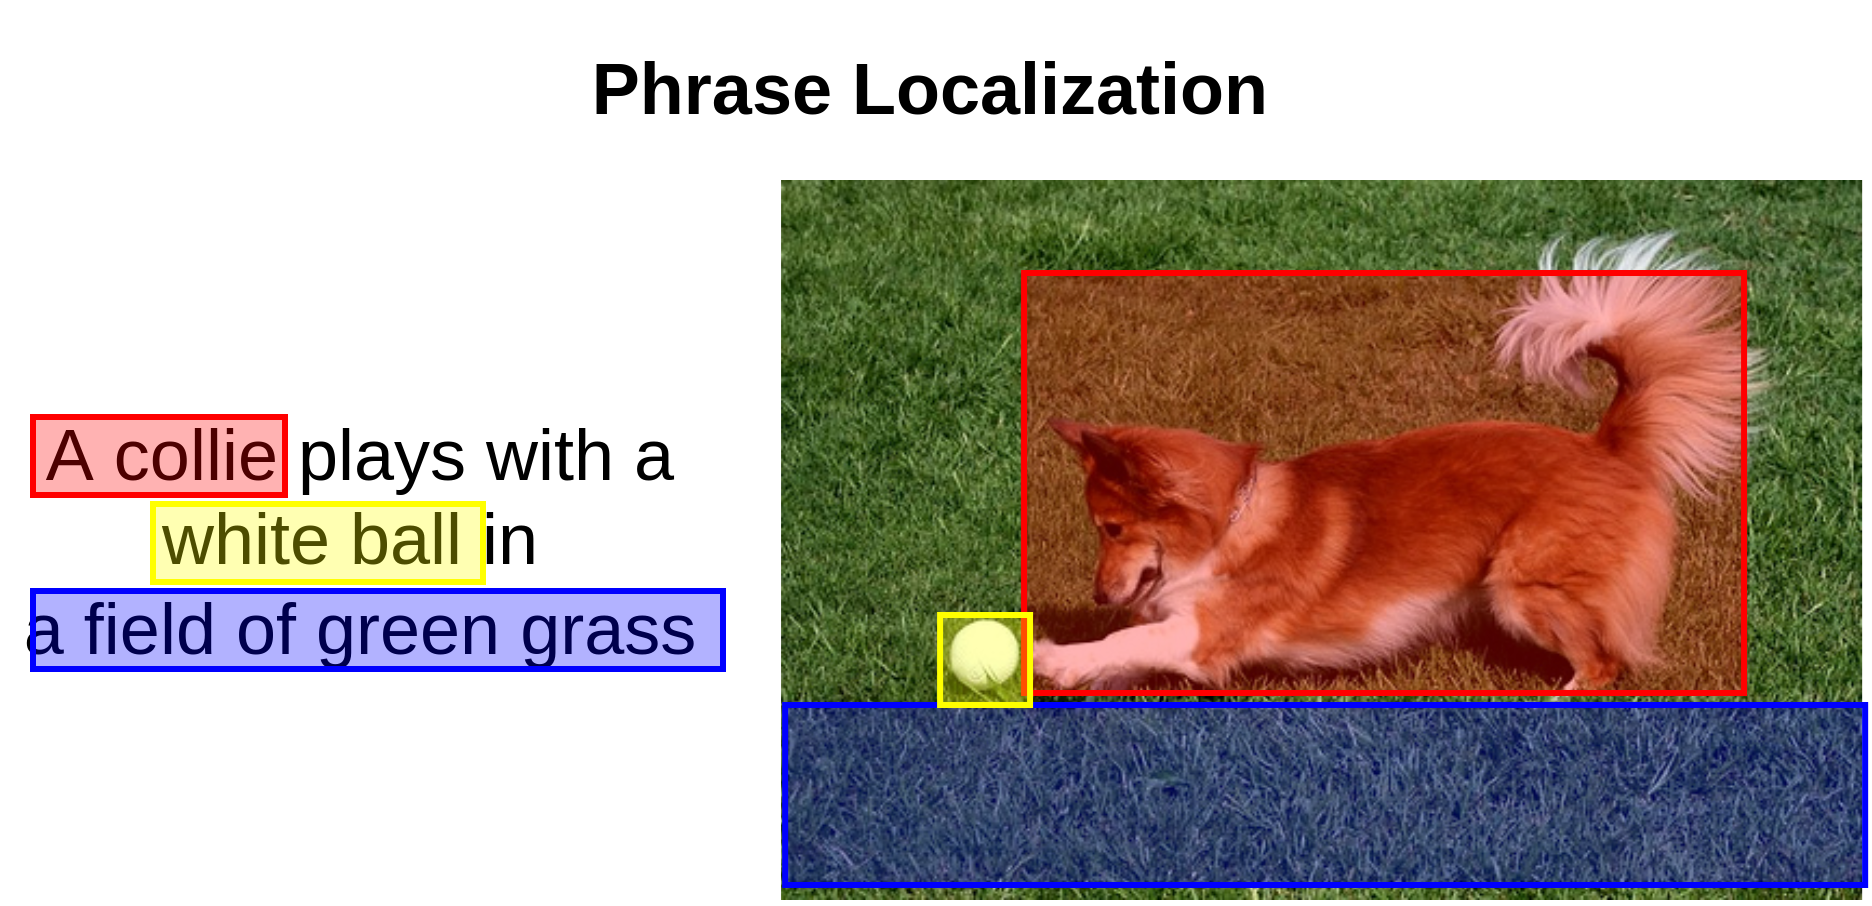
\includegraphics[width=7cm]{images/dog-playing-with-ball.png}

  \vspace{0.5cm}

  \begin{alertblock}{Def. (Phrase Grounding)}
    Attività di localizzazione del contenuto di un immagine referenziato da una
    frase.
  \end{alertblock}
\end{frame}

\section{Motivazione}

\begin{frame}{Motivazione}
  \begin{itemize}
    \item Tassello fondamentale per diversi task in computer vision
    \item Capire in modo più profondo come gli umani fanno phrase grounding
  \end{itemize}
\end{frame}

\section{Stato dell'arte}

\begin{frame}{Approcci}
  \begin{itemize}
    \item Sfruttare l'informazione contenuta nella \alert{struttura
    della frase}
    \item Riformulare il problema del phrase grounding sotto forma del
    task \alert{image retrieval}
    \item \alert{Ricostruire} le feature originali partendo da un
    codice (encoder-decoder)
  \end{itemize}
\end{frame}

\section{La nostra soluzione}

\begin{frame}{La nostra soluzione}
  \begin{itemize}
    \item Sfruttare informazione aggiuntiva dell'object detector (per
    ogni proposal restituisce una \alert{distribuzione di probabilità}
    su un set di classi)
    \item Le classi esprimono il \alert{contenuto semantico} delle
    proposal
    \item Data una frase ed una proposal, è più probabile che vi sia
    grounding tra le due se la \alert{similarità} tra la frase e la
    classe della proposal è alta
  \end{itemize}
\end{frame}

\begin{frame}{Architettura}
  \centering
  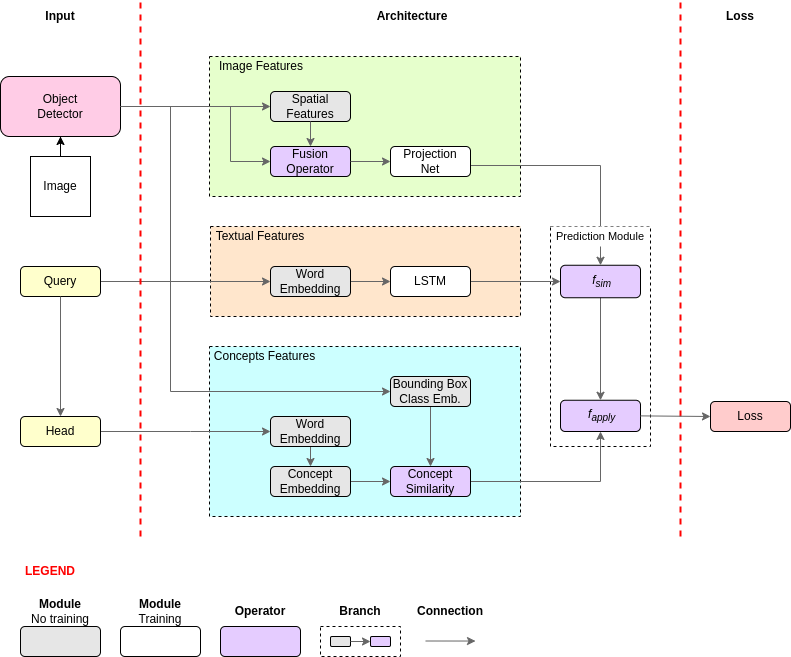
\includegraphics[width=9cm]{images/model-architecture.png}
\end{frame}

\begin{frame}{Similarità di concetto}
  \centering
  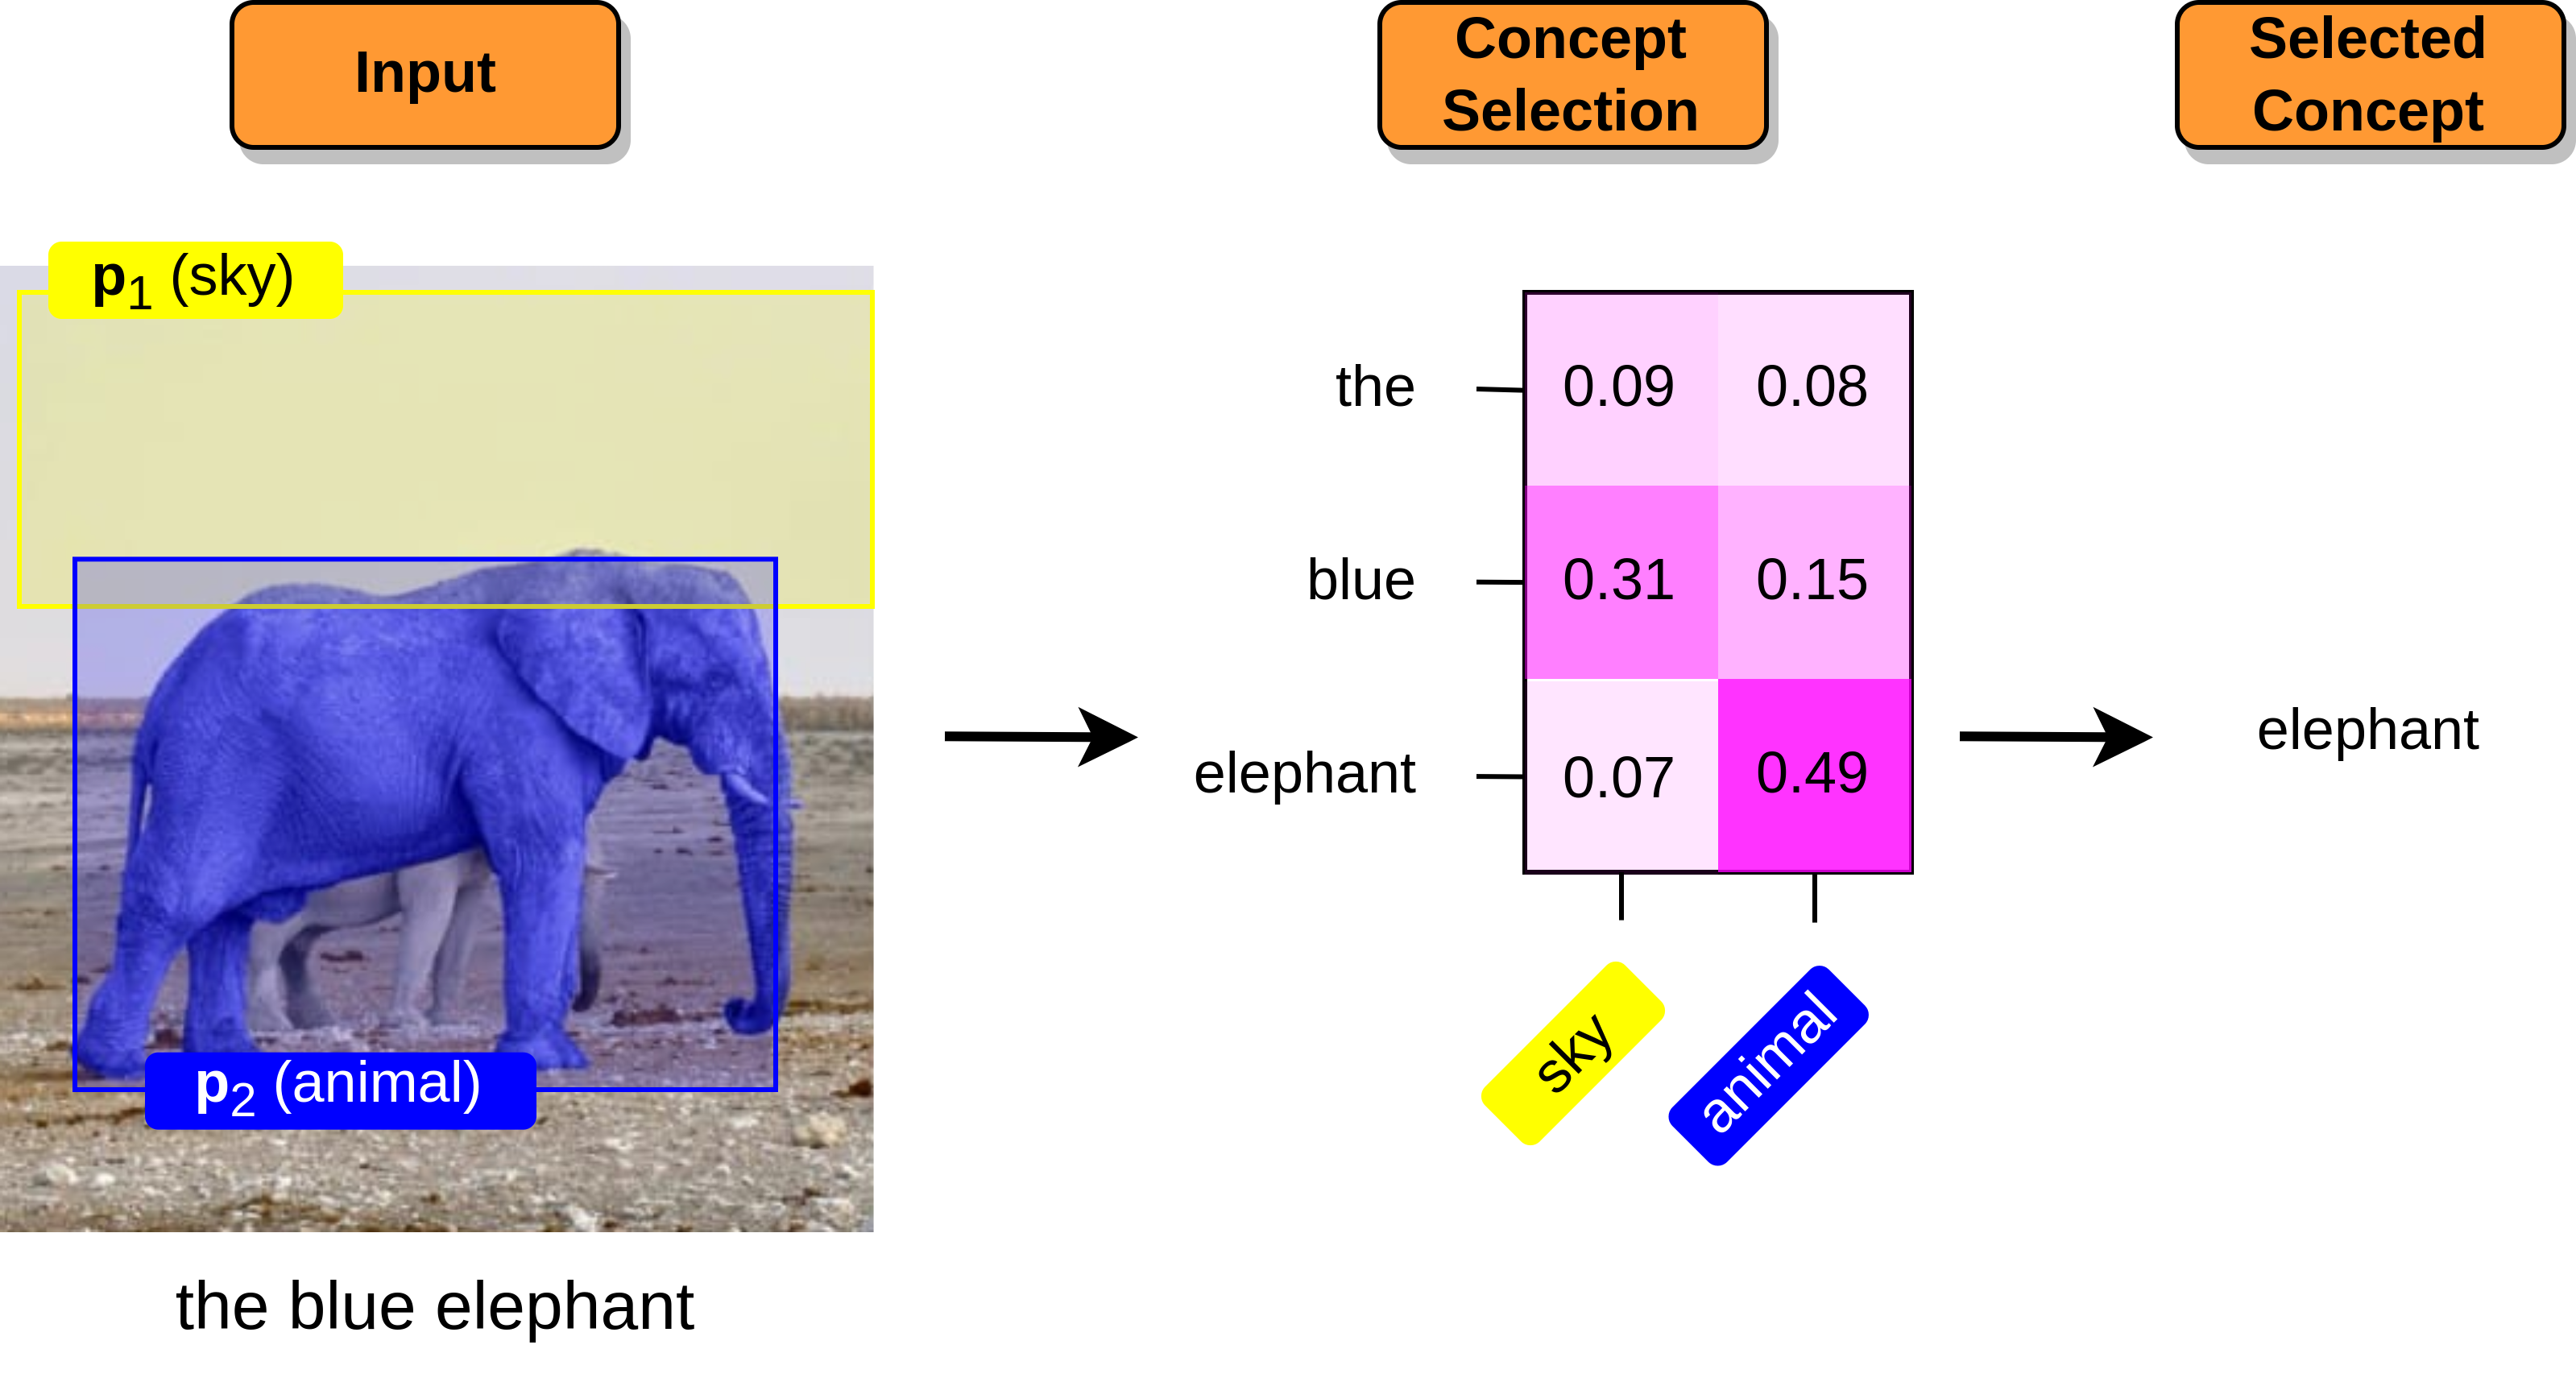
\includegraphics[width=9cm]{images/concept-selection-example.png}
\end{frame}

\begin{frame}{Predizioni}
  \centering
  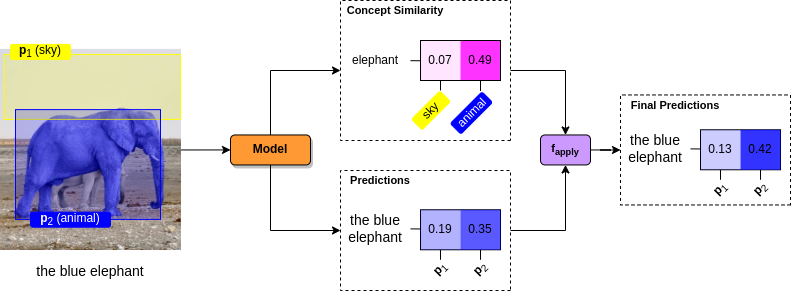
\includegraphics[width=10cm]{images/predictions.png}
\end{frame}

\begin{frame}{Loss}
  \centering
  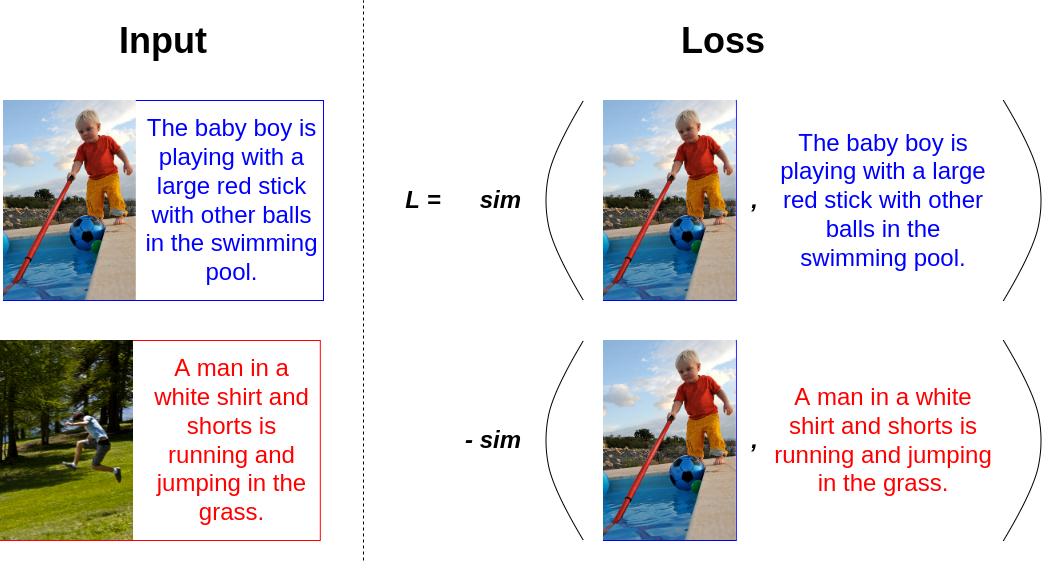
\includegraphics[width=9cm]{images/loss.png}
\end{frame}

\begin{frame}{Similarità Multimodale}
  \centering
  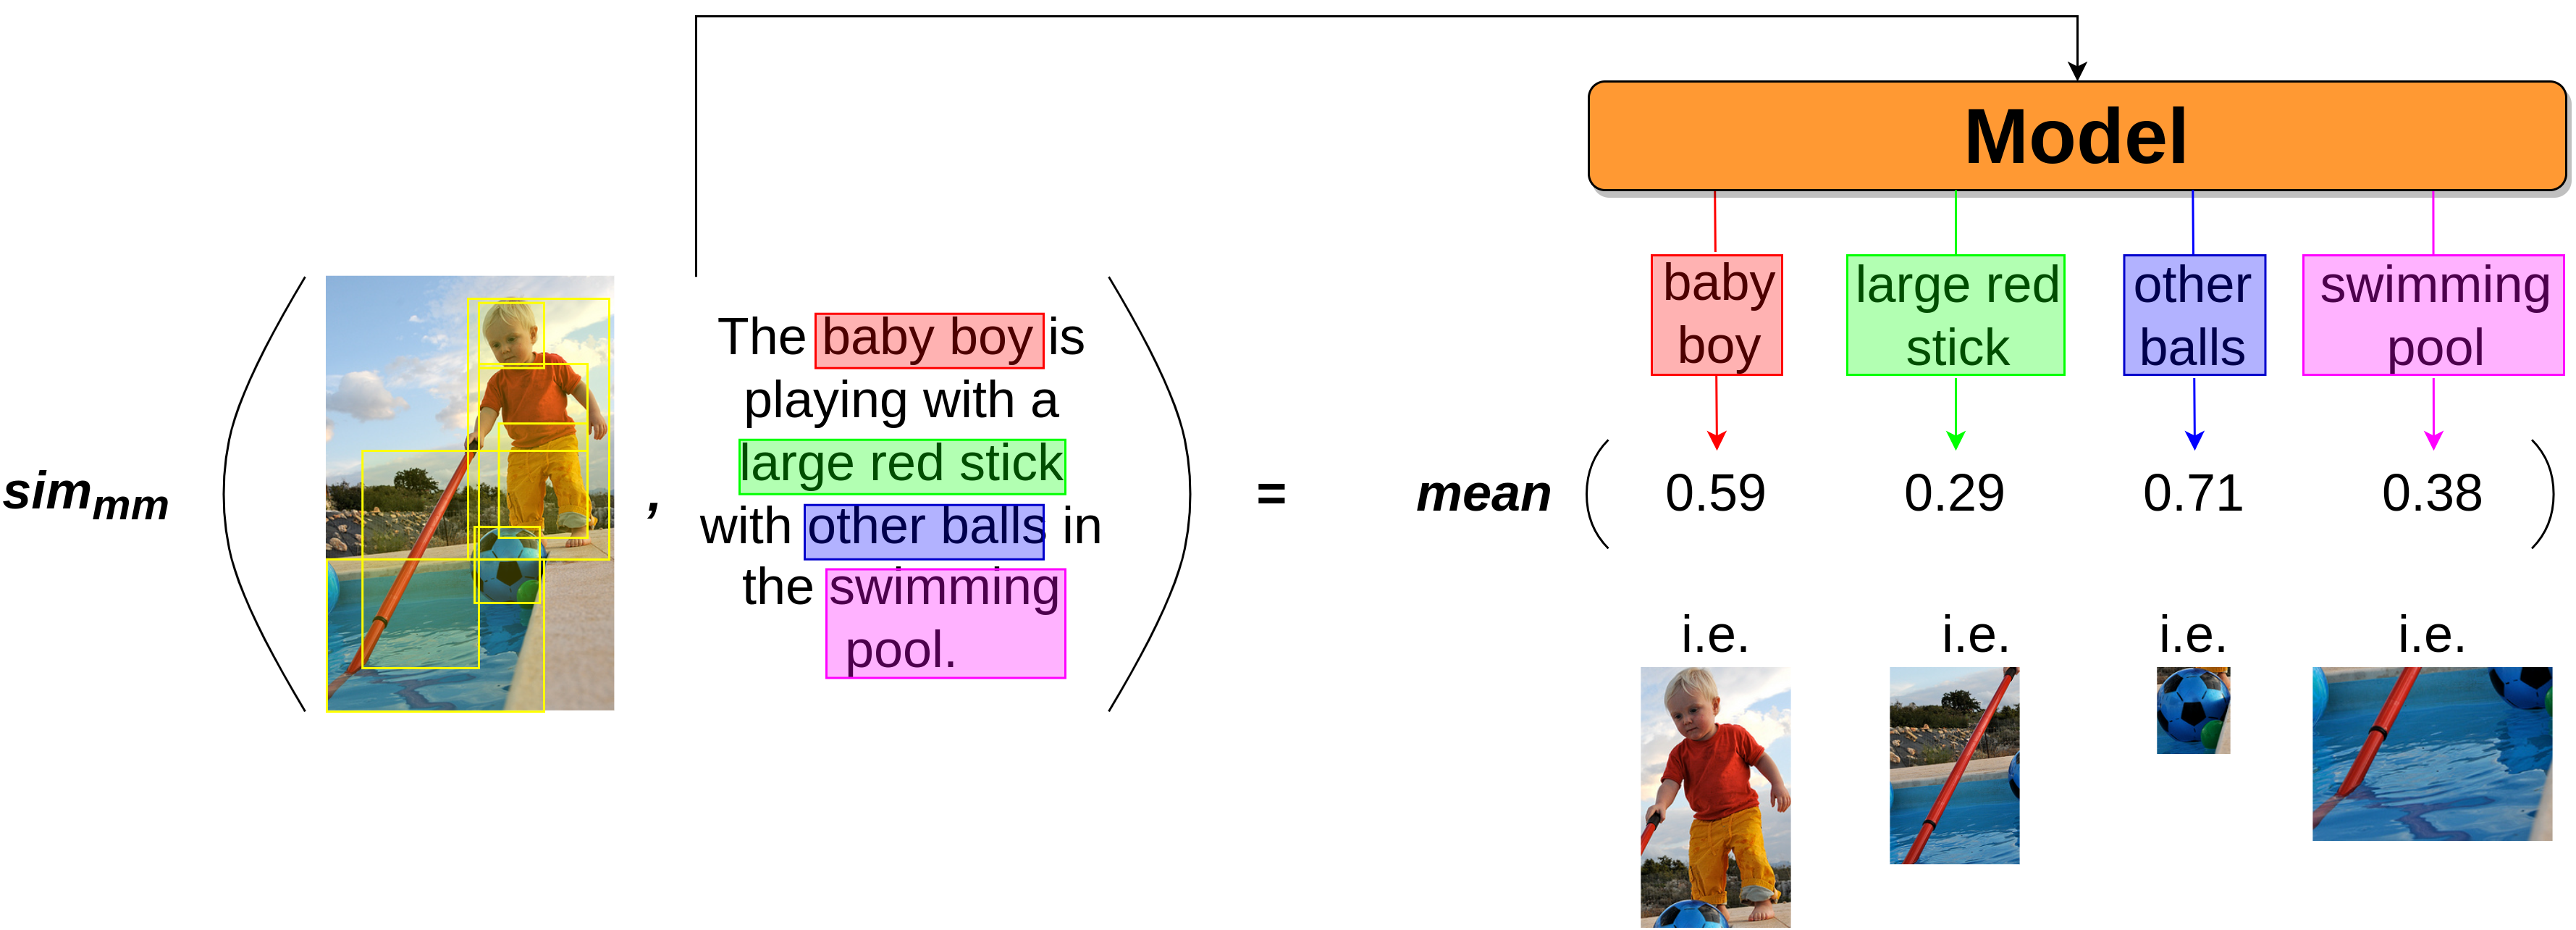
\includegraphics[width=9cm]{images/sim-mm.png}
\end{frame}

\begin{frame}{First section}
  \begin{block}{Normal block}
    Fusce luctus venenatis felis quis semper
  \end{block}

  \begin{alertblock}{Alert block}
    $$ E = (x_1 \vee \neg x_2 \vee \neg x_3) \wedge (x_1 \vee x_2 \vee x_4) $$
  \end{alertblock}

  \begin{exampleblock}{Example block}
    Proin tincidunt, neque at tincidunt mollis
  \end{exampleblock}
\end{frame}


\end{document}
